\begin{figure}[t]
\centering
% src: fig/supp_runs_fsc.pdf by scripts/paper_supp_timing.py; curves: docs/paper/supp_runs_fsc.csv (from runs/engine/pose_abc_adopt_20261113/blind/scores/cycle4/structure/curves.csv and runs/engine/abc_4090_20261117/scores/cycle4/structure/curves.csv)
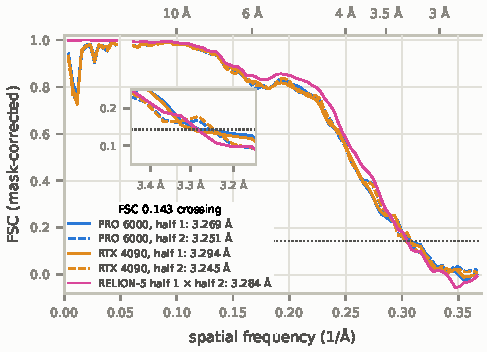
\includegraphics[width=\columnwidth]{fig/supp_runs_fsc.pdf}
\caption{\textbf{Run-to-run variation.} Final STAGS half maps of the PRO 6000 run (blue) and the RTX 4090 run (orange) against the opposite RELION-5 half map (solid: half 1, dashed: half 2), and RELION-5's own half 1 against half 2 (magenta); inset, 3.45--3.15\,\AA. Same scorer, grid and mask as \mainref{fig:fsc}.}
\label{fig:suppl:runs}
\end{figure}

\begin{table*}[t]
\centering
\footnotesize
\setlength{\tabcolsep}{5pt}
\resizebox{\textwidth}{!}{\begin{tabular}{@{}lccccc@{}}
\toprule
& FSC 0.143 crossing (\AA) $\downarrow$ & FSC at 3.5\,\AA\ $\uparrow$ & Mean FSC, 3.6--3.28\,\AA\ $\uparrow$ & Atomic FSC 0.5 (\AA) $\downarrow$ & Picks to final map (h) \\
\midrule
% generated by scripts/paper_supp_timing.py; csv: docs/paper/supp_timing_runs.csv
% src: runs/engine/pose_abc_adopt_20261113/blind/scores/cycle4/results.json; band: runs/engine/pose_abc_adopt_20261113/blind/scores/cycle4/structure/curves.csv; time: runs/engine/pose_abc_adopt_20261113/blind/report.json wall_min
STAGS, PRO 6000 & 3.269 / 3.251 & 0.247 / 0.243 & 0.228 / 0.226 & 4.04 & 4.27 \\
% src: runs/engine/abc_4090_20261117/scores/cycle4/results.json; band: runs/engine/abc_4090_20261117/scores/cycle4/structure/curves.csv; time: runs/engine/abc_4090_20261117/full_logs/report.json wall_min
STAGS, RTX 4090 & 3.294 / 3.245 & 0.252 / 0.266 & 0.228 / 0.234 & 4.01 & 4.39 \\
% src: runs/engine/a4_selftest_20261113_merge/i_relion_halves/results.json; band: runs/engine/a4_selftest_20261113_merge/i_relion_halves/structure/curves.csv; time: scripts/lean_chain.py RELION constants (its own logs, other hardware)
RELION-5 job078 & 3.284 / 3.284 & 0.276 / 0.277 & 0.244 / 0.244 & 3.86 & 24.1$^\ddagger$ \\
\bottomrule
\end{tabular}}
\caption{\textbf{Final maps of the two blind STAGS runs and of RELION-5 (polished).} Cross-FSC of half 1 / half 2 against the opposite RELION-5 half map (RELION-5: its own half 1 against half 2); atomic: FSC 0.5 of the half-map average against 5L93. $^\ddagger$RELION-5 tutorial logs, other hardware.}
\label{tab:suppl:runs}
\end{table*}

\begin{table}[t]
\centering
\footnotesize
\setlength{\tabcolsep}{3pt}
\begin{tabular}{@{}lrcrc@{}}
\toprule
& \multicolumn{2}{c}{PRO 6000} & \multicolumn{2}{c}{RTX 4090} \\
\cmidrule(lr){2-3}\cmidrule(lr){4-5}
After & min & FSC 0.143 (\AA) & min & FSC 0.143 (\AA) \\
\midrule
% generated by scripts/paper_supp_timing.py; csv: docs/paper/supp_timing_resolution.csv
% src (min): end of the stage on the run clock, from tab:suppl:stages sources (runs/engine/pose_abc_adopt_20261113/blind/lean/timing.json, runs/engine/abc_4090_20261117/full_logs/lean/timing.json, report.json, done/*.json)
% src: runs/engine/pose_abc_adopt_20261113/blind/lean/score_step1_seed/results.json; runs/engine/abc_4090_20261117/full_logs/lean/score_step1_seed/results.json
% scored after the run (lean timing.json stages.step1_seed.score_error: exit 1; see logs/score_step1_seed.log); runs/engine/abc_4090_20261117/full_logs/lean/logs/score_step1_seed.log
Seed, 16\,\AA & 15 & 14.131 / 14.236 & 9 & 14.107 / 14.201$^\S$ \\
% src: runs/engine/pose_abc_adopt_20261113/blind/lean/score_step2_16_12/results.json; runs/engine/abc_4090_20261117/full_logs/lean/score_step2_16_12/results.json
% scored after the run (lean timing.json stages.step2_16_12.score_error: exit 1; see logs/score_step2_16_12.log); runs/engine/abc_4090_20261117/full_logs/lean/logs/score_step2_16_12.log
Ladder 16/12\,\AA & 25 & 13.687 / 12.303 & 16 & 12.089 / 12.225$^\S$ \\
% src: runs/engine/pose_abc_adopt_20261113/blind/lean/score_step2_10/results.json; runs/engine/abc_4090_20261117/full_logs/lean/score_step2_10/results.json
% scored after the run (lean timing.json stages.step2_10.score_error: exit 1; see logs/score_step2_10.log); runs/engine/abc_4090_20261117/full_logs/lean/logs/score_step2_10.log
Ladder 10\,\AA & 34 & 9.623 / 9.772 & 22 & 9.474 / 9.559$^\S$ \\
% src: runs/engine/pose_abc_adopt_20261113/blind/lean/score_step3_8_6.5/results.json; runs/engine/abc_4090_20261117/full_logs/lean/score_step3_8_6.5/results.json
% scored after the run (lean timing.json stages.step3_8_6.5.score_error: exit 1; see logs/score_step3_8_6.5.log); runs/engine/abc_4090_20261117/full_logs/lean/logs/score_step3_8_6.5.log
Ladder 8/6.5\,\AA & 58 & 6.007 / 5.982 & 54 & 6.019 / 6.326$^\S$ \\
% src: runs/engine/pose_abc_adopt_20261113/blind/lean/score_step4_5.5/results.json; runs/engine/abc_4090_20261117/full_logs/lean/score_step4_5.5/results.json
Ladder 5.5\,\AA & 89 & 5.671 / 5.667 & 89 & 5.731 / 5.689 \\
% src: runs/engine/pose_abc_adopt_20261113/blind/scores/fit0/results.json; runs/engine/abc_4090_20261117/scores/fit0/results.json
Cold KB map fit & 113 & 3.904 / 4.063 & 113 & 3.935 / 4.063 \\
% src: runs/engine/pose_abc_adopt_20261113/blind/scores/cycle1/results.json; runs/engine/abc_4090_20261117/scores/cycle1/results.json
Cycle 1 & 150 & 3.370 / 3.403 & 153 & 3.372 / 3.433 \\
% src: runs/engine/pose_abc_adopt_20261113/blind/scores/cycle2/results.json; runs/engine/abc_4090_20261117/scores/cycle2/results.json
Cycle 2 & 186 & 3.325 / 3.362 & 190 & 3.312 / 3.231 \\
% src: runs/engine/pose_abc_adopt_20261113/blind/scores/cycle3/results.json; runs/engine/abc_4090_20261117/scores/cycle3/results.json
Cycle 3 & 222 & 3.307 / 3.243 & 227 & 3.294 / 3.241 \\
% src: runs/engine/pose_abc_adopt_20261113/blind/scores/cycle4/results.json; runs/engine/abc_4090_20261117/scores/cycle4/results.json
Cycle 4 & 256 & 3.269 / 3.251 & 263 & 3.294 / 3.245 \\
\bottomrule
\end{tabular}
\caption{\textbf{Resolution after each stage}: cross-FSC 0.143 crossing of half 1 / half 2 against the opposite RELION-5 half map, and the run clock at the end of the stage (min). RTX 4090 ladder rows marked $^\S$ were scored after the run with the same scorer (in the run, the scorer refused to start without its self-test on that machine); all scores are reporting only.}
\label{tab:suppl:resolution}
\end{table}
